

%Language and Encoding
\usepackage[francais]{babel}
\usepackage[utf8]{inputenc}

%Images
\usepackage{graphicx} 

%Algorithm 
\usepackage{algorithmic}
\usepackage{algorithm}


%Info
\title{\textbf{Contrôle d'accès e le POSIX Access Control Lists(ACL)} \\ CS435 - Administration de Système }
\author{Dan Pham et Fabrício Nascimento}
\date{Octobre 2009}

\begin{document}

\maketitle
\newpage
%----------------------------------------------------------------------------
\section*{Introduction}

%Le probleme et la solution plus simple
Quand l'objective c'est contrôle l'accès sur les données dans une système de fichiers, il y a plusieurs formes de règlement. Par défaut, les systèmes POSIX (Portable Operatin System Interface)\cite{ieee1,ieee2} ont une mécanisme que permettre de associer chaque entité avec un ensemble de règle, lequel est composé par une séquence d'octet que exprime le droit du propriétaire, de son groupe et des autres utilisateurs. 

%les limitation de ce solution la
Ce mode traditionnel est assez simple et capable de adresser les problème plus fréquents. Par contre, il pose des limitation aux administrateur de système, lesquels fréquemment doivent employer quelques configuration non évidentes afin d'être capable de exprimer ces besoins. Par exemple les application comme le serveur FTP Proftp\cite{ftp} ont ces exclusive façon de résoudre ces problèmes de droits pour accéder les objets du système de fichier.

% La solution ACL
À couse de remédier ces limitation présente les UNIX permettent d'employer les ACL.   

% Le reference aux texte originale
Cette article présente une exposition sur les ACL POSIX, ces mode de fonctionnement, ces clefs de succès et désavantages. Le texte est fortement basé en l'article de Andreas Gruembacher\cite{aclsuse} dont a été dans l'équipe que as ajouté le support aux ACL dans le noyaux Linux pour les système de fichier ext2 et ext3, lequel est le système de fichier plus utilisé dans les monde UNIX.


%----------------------------------------------------------------------------
\section{Le POSIX 1003.1}

%regarder bien le passer

Traditionnellement les système qui implémentions les patron POSIX avaient une système simple et puissante de permission, quand même, certain problèmes ont arrive, et éventuellement les problèmes ont apparaître. 

Après savoir la nécessite de régler sur le domaine de sécurise et non seulement les ACL, une groupe a était forme pendant la définition de la famille de patron POSIX 1003.1. Les premières documents POSIX qui ont été considère ces question étaient les document 1003.1e (\emph{System Application Programming Interface}) et 1003.2c (\emph{Shell and Utilities}), cependant, la première approximation de ce sujet était trop ambitieuse. Les groupe responsable pour le patronisation avait centre ces effort dans une tas assez grande de choses, lesquelles  comprenant \emph{Access Control Lists} (ACL), \emph{Audit}, \emph{Capability},\emph{ Mandatory Access Control }(MAC), et \emph{Information Labeling}\cite{aclsuse}.

En Janvier de 1998\cite{aclsuse} le financement était fini, par contre, le travaille n'était pas prés. De toute façon le dixsèptieme brouillon a été publique quand même\cite{posix17}.

Donc après cette an, les système UNIX appelé "\emph{trusted}" (Trusted Solaris, Trusted Irix, Trusted AIX ont été développer avec quelque parts de la documentation 17. Ces systèmes ne sont pas complètement compatible entre eux. 

Aujourd'hui la plupart des système UNIX et UNIX-like support ACL. Ces implémentassions sont usuellement compatible avec le document 17. Le projet TrustedBSD aussi avait ajouter les ACL sur les système BSD. Les ACL e les MAC  FreeBSD-RELEASE avaient apparu en 2003.

Les base des ACL sont lancé sur le système traditionnel présent usuellement dans presque tous les système UNIX, alors, avant de préciser sur les ACL on parlerais du modelé traditionnel.

\subsection*{Système de permission Traditionnel}

%Les groups e les permission
Le modelé traditionnel POSIX offre trois group de utilisateur qui sont le propriétaire, le group e les autres. Chaque group a une octet que indique les permission de lecture (\textbf{r}ead), écrire (\textbf{w}rite) et exécution (e\textbf{x}ecute). La première classe fournit les permission pour le utilisateur que rempli le rôle de propriétaire, ensuite, vient les droits pour le groupe principal du propriétaire enfin les droites pour touts les autres utilisateurs. 
 
%Explication simple
Après les trois octets peut venir le \emph{Set User Id}, \emph{Set Group Id} et \emph{Sticky bit}, lesquelles sont utilisé dans certain cases. Il faut faire attention avec le \emph{Sticky Bit}, il permit les utilisateur normale d'exécuter les utilitaire comment le administrateur(\emph{root}), par contre, quelque manque de sécurité peut compromettre le système entière.

%Le droit du root
Seulement le \emph{root} peut créer les groups e changer les association de groupes. Celui-là que aussi peut changer les propriétaire. 

\subsection*{Les ACL}

%Basic Definitions
Dans une modèle de de sécurise ACL, si quelque agent faire une requête pour accéder aux donnés, il faut consulte les ACL pour une entrée que permettre l'opération demandé. Chaque ACL est une ensemble de règles d'accès. Les règles possible peut-être regarder dans le tableau ci-dessous\ref{entree}.
\begin{center}
\begin{tabular}{|l|l|}
  \hline
    \multicolumn{2}{|c|}{Les types de ACL} \\
  \hline
	\textbf{Type d'entrée} & \textbf{format} \\
  \hline
	Propriétaire & user::rwx \\
	Utilisateur nommée & user:name:rwx  \\
	Groupe propriétaire & group::rwx \\
	Groupe nommée & group:name:rwx \\
	Masque & mask::rwx \\
	Autres & other::rwx \\   
  \hline
\end{tabular}
\label{tab:entree}
\end{center}

Le format des règles sont formée par une indicateur de classe (comme les classe du système Traditionnel), une quantificateur pour spécifier de quel utilisateur ou group on parle et les octet de permission.

%EXPLIQUER MELLEIUR
Avec cette représentation le sens de la classe du groupe a redéfini comment le limite supérieur de les permission de chaque entrée dans la classe du groupe. Ça arrive parce que les entrée du groupe et du utilisateur nommées seront désigner à entrée du groupe. Aussi, c'est importante rappeler que cette choix permettre se prémunir contre les application qui ne sont pas conscient de les ACL.
\footnote{Fabricio: Je ne comprend pas cette affirmation, je laisse ici le teste orignial: 
These named group and named user entries are assigned to the group class, which already contains the owning group entry. Different from the POSIX.1 permission model, the group class may now contain ACL entries with different permission sets, so the group class permissions alone are no longer sufficient to represent all the detailed permissions of all ACL entries it contains. Therefore, the meaning of the group class permissions is redefined: under their new semantics, they represent an upper bound of the permissions that any entry in the group class will grant. This upper bound property ensures that POSIX.1 applications that are unaware of ACLs will not suddenly and unexpectedly start to grant additional permissions once ACLs are supported.}.

Les ACL qui sont équivalent avec le mode simple de permission de fichier s'appellent minimale et ils ont trois entrée. Si les ACL peut avoir plusieurs entrée ont les appelle étendu. Tous les ACL étendu doivent avoir l'entrée masque et peut contenir théoriquement n'importe combien de entrée. On verrais après que ce numéro d'entrée peut-être limitée pour chaque implémentassions et que aussi il est important pour la performance.

%EXPLIQUER MELLEIUR
Dans les ACL minimale les permission de classe groupe sont égale à les permission de groupe propriétaire, cependant, dans les ACL étendu on peut avoir les entrée avec plusieurs utilisateurs et/ou groupes, quelques de cette entrées peut-être contenir permissions qui la classe groupe n'aurais pas, alors, on peut avoir une inconsistance basée en le cas qui les permissions du groupe propriétaire sont diffèrent de les permission de la classe groupe. 

On résoudre ce problème avec le masque. Comme on peut observer dans le figure 1\ref{fig:img_acl-mapping}, il y a deux cas: les permission de la classe groupe seront déguise pour la masque tandis que les permission de l'entrée du groupe propriétaire encore définit les permission pour le groupe propriétaire.    


\begin{figure}[htbp]
	\centering
		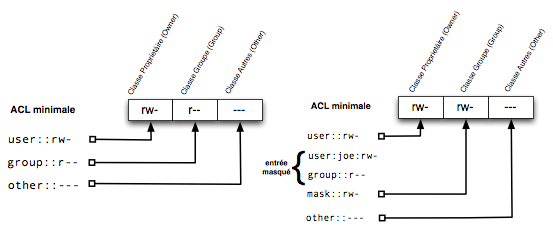
\includegraphics[height=3in]{img/acl-mapping.jpg}
	\caption{caption}
	\label{fig:img_acl-mapping}
\end{figure}


Pour assurer le consistance, quand une application change les permission (par exemple le commande \emph{chmod}) les ACL sont modifiée de façon a reproduire ce modification. 



% Explication plus precise sur les masque 
%
% The group class permissions represent the upper bound of the permissions granted by any entry in the group class. With minimal ACLs this is trivially the case. With extended ACLs, this is implemented by masking permissions (hence the name of the mask entry): permissions in entries that are a member of the group class which are also present in the mask entry are effective. Permissions that are absent in the mask entry are masked and thus do not take effect. See Table 2.
% 
% 
% Table: Masking of Permissions
% Entry type 	Text form 	Permissions
% Named user 	user:joe:r-x 	r-x
% Mask 	mask::rw- 	rw-
% Effective permissions 	r-
% 
% 
% The owner and other entries are not in the group class. Their permissions are always effective and never masked.
% 
% 

\subsection*{Algorithme de vérification}

Pour vérifier les droits d'accès de une objet du système de fichier il y a une algorithme assez simple. 

%changer le titre et la langue
\begin{algorithm}
\caption{Vérifie se une utilisateur peut ou ne peut pas accéder une objet du système de fichier}
\label{algacl}
\begin{algorithmic}
\IF{the user ID of the process is the owner}
	\STATE the owner entry determines access
\ELSIF{the user ID of the process matches the qualifier in one of the named user entries}
	\STATE this entry determines access 
\ELSIF{one of the group IDs of the process matches the owning group and the owning group entry contains the requested permissions} 
	\STATE this entry determines access
\ELSIF{one of the group IDs of the process matches the qualifier of one of the named group entries and this entry contains the requested permissions}
	\STATE this entry determines access
 
\ELSIF{one of the group IDs of the process matches the owning group or any of the named group entries, but neither the owning group entry nor any of the matching named group entries contains the requested permissions} 
\STATE this determines that access is denied

\ELSE
	\STATE the other entry determines access.
\ENDIF
 

\IF{the matching entry resulting from this selection is the owner or other entry and it contains the requested permissions}
	\STATE access is granted 
\ELSIF{the matching entry is a named user, owning group, or named group entry and this entry contains the requested permissions and the mask entry also contains the requested permissions (or there is no mask entry)}
	\STATE access is granted
 
\ELSE
	\STATE access is denied.
\ENDIF
\end{algorithmic}
\end{algorithm}


\subsection*{Héritage mécanisme}


% 
% So far we have only looked at ACLs that define the current access permissions of file system objects. This type is called access ACL. A second type called default ACL is also defined. They define the permissions a file system object inherits from its parent directory at the time of its creation. Only directories can be associated with default ACLs. Default ACLs for non-directories would be of no use, because no other file system objects can be created inside non-directories. Default ACLs play no direct role in access checks.
% 
% When a directory is created inside a directory that has a default ACL, the new directory inherits the parent directory's default ACL both as its access ACL and default ACL. Objects that are not directories inherit the default ACL of the parent directory as their access ACL only.
% 
% The permissions of inherited access ACLs are further modified by the mode parameter that each system call creating file system objects has. The mode parameter contains nine permission bits that stand for the permissions of the owner, group, and other class permissions. The effective permissions of each class are set to the intersection of the permissions defined for this class in the ACL and specified in the mode parameter.
% 
% If the parent directory has no default ACL, the permissions of the new file are determined as defined in POSIX.1. The effective permissions are set to the permissions defined in the mode parameter, minus the permissions set in the current umask.
% 
% The umask has no effect if a default ACL exists. 



\section{Linux}

%A voir maintenant
\subsection*{ACL Implementation in Linux}

%noyaux patches

% ls -l

%getfacl

%setfacl

%systemes de fichier

% Patches that implement POSIX 1003.1e draft 17 ACLs have been available for various versions of Linux for several years now. They were added to version 2.5.46 of the Linux kernel in November 2002. Current Linux distributions are still based on the 2.4.x stable kernels series. SuSE and the United Linux consortium have integrated the 2.4 kernel ACL patches earlier than others, so their current products offer the most complete ACL support available for Linux to date. Other vendors apparently are still reluctant to make that important change, but experimental versions are expected to be available later this year.
% 
% The Linux getfacl and setfacl command line utilities do not strictly follow POSIX 1003.2c draft 17, which shows mostly in the way they handle default ACLs. See section 6.
% 
% At the time of this writing, ACL support on Linux is available for the Ext2, Ext3, IBM JFS, ReiserFS, and SGI XFS file systems. Solaris-compatible ACL support for NFS version 3 exists since March 3, 2003.

%----------------------------------------------------------------------------

\section*{Conclusion}

\begin{thebibliography}{9}
 
\bibitem{aclsuse}
  Andreas Gruenbacher,
  \emph{POSIX Acess Control Lists on Linux}.
  http://www.suse.de/~agruen/acl/linux-acls/online/,
  2003.

\bibitem{ieee1}
    IEEE Std 1003.1-2001 (Open Group Technical Standard, Issue 6), 
	Standard for Information Technology--Portable Operating System Interface (POSIX) 2001. 
	ISBN 0-7381-3010-9. 
	http://www.ieee.org/

\bibitem{ieee2}
    IEEE 1003.1e and 1003.2c: Draft Standard for Information Technology--Portable Operating System Interface (POSIX)--Part 1: System Application Program Interface (API) and Part 2: Shell and Utilities, draft 17 (withdrawn). 
	October 1997. 
	http://wt.xpilot.org/publications/posix.1e/

\bibitem{ftp}
	Mark Lowes: 
	Proftpd: 
	A User's Guide March 31, 2003. 
	http://proftpd.linux.co.uk/

\bibitem{posix17}
    Winfried Trümper: Summary about Posix.1e. Publicly available copies of POSIX 1003.1e/1003.2c. February 28, 1999. http://wt.xpilot.org/publications/posix.1e/

\end{thebibliography}

\end{document}